\documentclass[pdflatex,sn-mathphys-num]{sn-jnl}

\usepackage{graphicx}
\usepackage{multirow}
\usepackage{amsmath,amssymb,amsfonts}
\usepackage{amsthm}
\usepackage{mathrsfs}
\usepackage[title]{appendix}
\usepackage{xcolor}
\usepackage{textcomp}
\usepackage{manyfoot}
\usepackage{booktabs}
\usepackage{algorithm}
\usepackage{algorithmicx}
\usepackage{algpseudocode}
\usepackage{listings}

\raggedbottom

\begin{document}

\title[Clasificación de Aptitud Solar: EDA y Diseño Experimental]{Clasificación de la Aptitud Solar Fotovoltaica a Partir de Variables Geoespaciales y Climáticas: Análisis Exploratorio de Datos y Diseño Experimental (Primera Entrega)}

\author*[1]{\fnm{Jesús David} \sur{Arévalo Montilla}}\email{jdarevalo@uninorte.edu.co}

\author[1]{\fnm{Enmanuel David} \sur{Diaz Molinares}}\email{denmanuel@uninorte.edu.co}

\author[1]{\fnm{Alex David} \sur{Teran Meza}}\email{talex@uninorte.edu.co}

\affil*[1]{\orgdiv{Departamento de Matemáticas y Ciencia de Datos, Programa de Ciencia de Datos}, \orgname{Universidad del Norte}, \orgaddress{\city{Barranquilla}, \country{Colombia}}}

\abstract{El dimensionamiento de infraestructura solar fotovoltaica a escala global requiere identificar con rapidez qué ubicaciones son aptas para la inversión, una decisión que hoy se apoya principalmente en simulaciones físicas puntuales (p. ej. PVGIS, Global Solar Atlas) costosas de escalar a miles de sitios candidatos. Este trabajo constituye la primera entrega de un proyecto de aprendizaje automático orientado a clasificar la aptitud solar de un sitio (Alta, Media o Baja) a partir de variables de terreno y clima disponibles antes de invertir, usando el conjunto de datos público \textit{Global Solar Power Plants Dataset} (\texttt{cimejia/solarPV}, 58{,}978 plantas en 183 países). Se presenta un pipeline de extracción, transformación y carga (ETL) y un Análisis Exploratorio de Datos (EDA) exhaustivo. El EDA reveló un desbalance de clases severo (Alta 75.10\%, Media 21.69\%, Baja 3.21\%), ausencia de duplicados, un sesgo geográfico marcado (10 países concentran el 79.8\% de las plantas) con la clase minoritaria concentrada casi exclusivamente en cuatro países europeos, ausencia de multicolinealidad relevante entre las 13 variables numéricas predictoras (VIF máximo de 4.29), y un chequeo de fuga de datos que descarta una relación estadística fuerte entre el target y variables posteriores a la inversión como \texttt{capacity} o \texttt{pv\_potential}. A partir de estos hallazgos se derivan decisiones de preprocesamiento concretas: métricas sensibles al desbalance, codificación cíclica de variables angulares, y una estrategia de validación cruzada espacial por país. Esta entrega establece la base de datos y metodológica sobre la cual se construirán, en entregas posteriores, los modelos de referencia y el modelo propuesto del proyecto.}

\keywords{Aptitud solar fotovoltaica, Clasificación multiclase desbalanceada, Análisis Exploratorio de Datos, Sesgo de cobertura geográfica, Validación cruzada espacial}

\maketitle

\section{Introducción}\label{sec:intro}

La transición energética depende, en buena medida, de identificar con rapidez qué ubicaciones del planeta ofrecen condiciones adecuadas para instalar infraestructura solar fotovoltaica antes de comprometer capital en estudios de sitio. Las herramientas de referencia actuales, como PVGIS o el Global Solar Atlas, se apoyan en modelos físicos de transferencia radiativa y bases meteorológicas satelitales que, aunque precisas, requieren una consulta puntual por ubicación y no están pensadas para evaluar simultáneamente miles de sitios candidatos. Un modelo de aprendizaje automático entrenado sobre variables de terreno y clima ampliamente disponibles (elevación, pendiente, orientación, temperatura, irradiancia, viento) ofrece una alternativa complementaria: una función de clasificación evaluable en milisegundos que etiquete cada sitio como de aptitud Alta, Media o Baja, sin ejecutar una simulación física completa por consulta.

Este proyecto usa el conjunto \textit{Global Solar Power Plants Dataset} \cite{bib1}, desarrollado conjuntamente por la Universidad de Alicante y la Universidad Central del Ecuador, que integra 58{,}978 plantas solares de 183 países con variables geoespaciales, de terreno, meteorológicas, y un índice compuesto de aptitud solar calculado por los autores originales. A diferencia de un enfoque de regresión sobre un potencial fotovoltaico continuo, este trabajo plantea el problema como clasificación multiclase ordinal sobre la categoría de aptitud (\texttt{solar\_aptitude\_class}: Baja, Media, Alta) ya provista por el dataset, una formulación más directamente alineada con la pregunta de negocio que motiva el proyecto (¿vale la pena invertir en este sitio?), aunque exige tratar con cuidado un desbalance de clases pronunciado.

El dataset presenta tres retos metodológicos que motivan esta primera entrega. Primero, un desbalance de clases severo: la categoría Baja representa apenas una fracción marginal del total, lo que puede hacer que un clasificador ingenuo parezca competente sin distinguir esa clase en absoluto si se evalúa únicamente por exactitud global \cite{bib3}. Segundo, un sesgo de cobertura geográfica hacia un puñado de países, que puede llevar a una partición aleatoria de entrenamiento y prueba a sobreestimar la capacidad de generalización del modelo hacia regiones subrepresentadas \cite{bib2}. Tercero, columnas derivadas de la construcción de la planta (\texttt{capacity}, \texttt{optimal\_tilt}, \texttt{pv\_potential}) cuyo uso indebido como predictoras constituiría fuga de datos, al no estar disponibles para un sitio que aún no ha sido construido ni evaluado.

Frente a estas limitaciones, la contribución de esta primera entrega es doble. Primero, se documenta un pipeline de ETL reproducible que valida el esquema, los tipos de datos y los rangos físicos del dataset. Segundo, se presenta un Análisis Exploratorio de Datos exhaustivo (univariado, bivariado, geográfico y de multicolinealidad) que cuantifica cada uno de los tres retos mencionados y traduce cada hallazgo en una decisión de preprocesamiento concreta y justificada. En este trabajo presentamos el EDA completo del \textit{Global Solar Power Plants Dataset} bajo un enfoque de clasificación, y mostramos con evidencia cuantitativa por qué una partición aleatoria y un conjunto de predictoras sin depurar conducirían a estimaciones de desempeño optimistas y poco fiables; las decisiones derivadas de este análisis son el punto de partida sobre el cual, en las siguientes entregas, se entrenarán y compararán los modelos de clasificación del proyecto.

\section{Planteamiento del problema}\label{sec:planteamiento}

El problema abordado es de \textbf{clasificación supervisada multiclase} \cite{bib3}. Dado un vector de variables predictoras $x$ que describe la geolocalización, el terreno y el clima de un punto del planeta,

\begin{equation}
\begin{split}
x = \big(\ &\text{longitud},\ \text{latitud},\ \text{elevación},\ \text{área},\ \text{pendiente},\ \text{tipo de pendiente},\\
&\text{curvatura},\ \text{tipo de curvatura},\ \text{aspecto},\ \text{tipo de aspecto},\ \text{distancia a vía},\\
&\text{temperatura},\ \text{irradiancia},\ \text{humedad},\ v_{\text{viento}},\ d_{\text{viento}},\ \text{dirección predom. del viento}\ \big),
\end{split}
\label{eq:features}
\end{equation}

\noindent se busca aprender una función de clasificación $f_\theta$ que asigne a cada sitio su clase de aptitud solar,

\begin{equation}
\hat{y} = f_\theta(x) \in \{\text{Baja}, \text{Media}, \text{Alta}\}, \qquad \theta^* = \arg\min_{\theta} \; \mathbb{E}_{(x,y)\sim \mathcal{D}}\left[ \mathcal{L}(f_\theta(x), y) \right],
\label{eq:objetivo}
\end{equation}

\noindent donde $\mathcal{D}$ es la distribución conjunta de variables predictoras y clase de aptitud observada en el dataset, y $\mathcal{L}$ es una función de pérdida de clasificación sensible al desbalance entre clases (p. ej. entropía cruzada ponderada por clase), que se definirá formalmente junto con las métricas de evaluación en la entrega de resultados. La variable $y$ es categórica ordinal de 3 niveles y está fuertemente desbalanceada (Sección~\ref{subsec:eda}), lo que descarta evaluar el modelo únicamente por exactitud global.

\section{Metodología de datos}\label{sec:metodologia}

Esta sección documenta el conjunto de datos utilizado, el pipeline de ETL aplicado y el Análisis Exploratorio de Datos realizado sobre las 58{,}978 plantas del dataset.

\subsection{Descripción general del dataset}\label{subsec:datos}

Se utiliza el \textit{Global Solar Power Plants Dataset} (\texttt{cimejia/solarPV}) \cite{bib1}, desarrollado por investigadores del Departamento de Tecnología Informática de la Universidad de Alicante y de la Facultad de Ingeniería en Geología, Minas, Petróleos y Ambiental (FIGEMPA) de la Universidad Central del Ecuador, distribuido bajo licencia CC BY-NC 4.0. El dataset contiene $N = 58{,}978$ plantas solares y 29 columnas originales.

La variable objetivo es \texttt{solar\_aptittude\_class} (el nombre de columna conserva un typo heredado de la fuente original), categórica ordinal de 3 niveles: Alta (44{,}295 plantas, 75.10\%), Media (12{,}791, 21.69\%) y Baja (1{,}892, 3.21\%). Las 17 variables predictoras, resumidas en la Ecuación~\eqref{eq:features}, combinan información geográfica (\texttt{longitude}, \texttt{latitude}, \texttt{elevation}), de terreno (\texttt{area}, \texttt{slope}/\texttt{slope\_type}, \texttt{curvature}/\texttt{curvature\_type}, \texttt{aspect}/\texttt{aspect\_type}, \texttt{dist\_to\_road}) y meteorológica (\texttt{ambient\_temperature}, \texttt{ghi}, \texttt{humidity}, \texttt{wind\_speed}, \texttt{wind\_direction}, \texttt{dt\_wind}); 13 son numéricas y 4 categóricas.

Se excluyen del conjunto de predictoras \texttt{solar\_aptitude} y \texttt{solar\_aptitude\_rounded} (definen el target por binning), \texttt{capacity}, \texttt{optimal\_tilt} y \texttt{pv\_potential} (resultado de haber construido y configurado la planta), \texttt{operational\_status} (posterior a la decisión de inversión), y los identificadores \texttt{OBJECTID}, \texttt{code} y \texttt{plant\_name}. Dos variables adicionales, \texttt{size} (categórica: \texttt{Small}/\texttt{Medium}/\texttt{Big}) y \texttt{country} (183 categorías), se analizan en la Sección~\ref{subsec:eda} sin incorporarse todavía al conjunto de predictoras, a la espera de decidir su codificación.

\subsection{Extracción, Transformación y Carga (ETL)}\label{subsec:etl}

\textbf{Extract.} Los datos se extraen desde \texttt{Dataset\_Mundial\_Final.xlsx}, una copia de trabajo del \textit{Global Solar Power Plants Dataset} \cite{bib1}, cargada directamente con \texttt{pandas.read\_excel}.

\textbf{Transform.} Se validó que las 29 columnas esperadas estuvieran presentes, sin columnas adicionales, y que las 18 columnas numéricas relevantes tuvieran tipo de dato numérico tras la carga; ninguna requirió corrección. No se detectaron filas ni códigos de planta duplicados entre las 58{,}978 instancias. La validación de rangos físicos encontró una única violación: 1{,}105 registros (1.87\%) de \texttt{aspect} fuera de $[0^\circ, 360^\circ]$, que coinciden exactamente con las 1{,}105 plantas de la categoría \texttt{Flat} en \texttt{aspect\_type}; se trata de un valor centinela ($-1$) para terreno sin orientación definida, no un error de captura, y se tratará como categoría propia en el modelado. Las variables angulares \texttt{aspect} y \texttt{wind\_direction} se codificaron adicionalmente de forma cíclica (seno/coseno), necesario porque $0^\circ$ y $359^\circ$ representan orientaciones casi idénticas que un modelo lineal interpretaría como extremos opuestos. La única columna con valores faltantes es \texttt{area} (16{,}329 nulos, 27.69\%); su imputación queda pendiente para la etapa de modelado y no se resuelve en esta entrega.

\textbf{Load.} Tras la validación, el dataset conserva las 58{,}978 filas originales, con tipos de dato correctos en las 13 variables numéricas y el target. La semilla aleatoria se fija en \texttt{RANDOM\_STATE=42}. La partición de entrenamiento y prueba, que deberá ser estratificada por clase y agrupada espacialmente por país (Sección~\ref{subsec:geografico}), se definirá en la siguiente entrega una vez fijado el conjunto final de predictoras.

\subsection{Análisis Exploratorio de Datos (EDA) exhaustivo}\label{subsec:eda}

\subsubsection{Análisis univariado: variable objetivo}\label{subsec:univ_target}

Como se indicó en la Sección~\ref{subsec:datos}, la distribución de \texttt{solar\_aptittude\_class} está fuertemente desbalanceada: 75.10\% Alta, 21.69\% Media y 3.21\% Baja (razón Alta:Baja de 23.4:1), mostrada en la Figura~\ref{fig:clases}. Un modelo evaluado únicamente por exactitud global podría alcanzar cerca del 75\% de acierto sin distinguir un solo caso de Baja, por lo que las métricas de evaluación deben ponderar las clases por igual (F1 macro, recall por clase) y la partición de datos debe ser estratificada.

\begin{figure}[h]
\centering
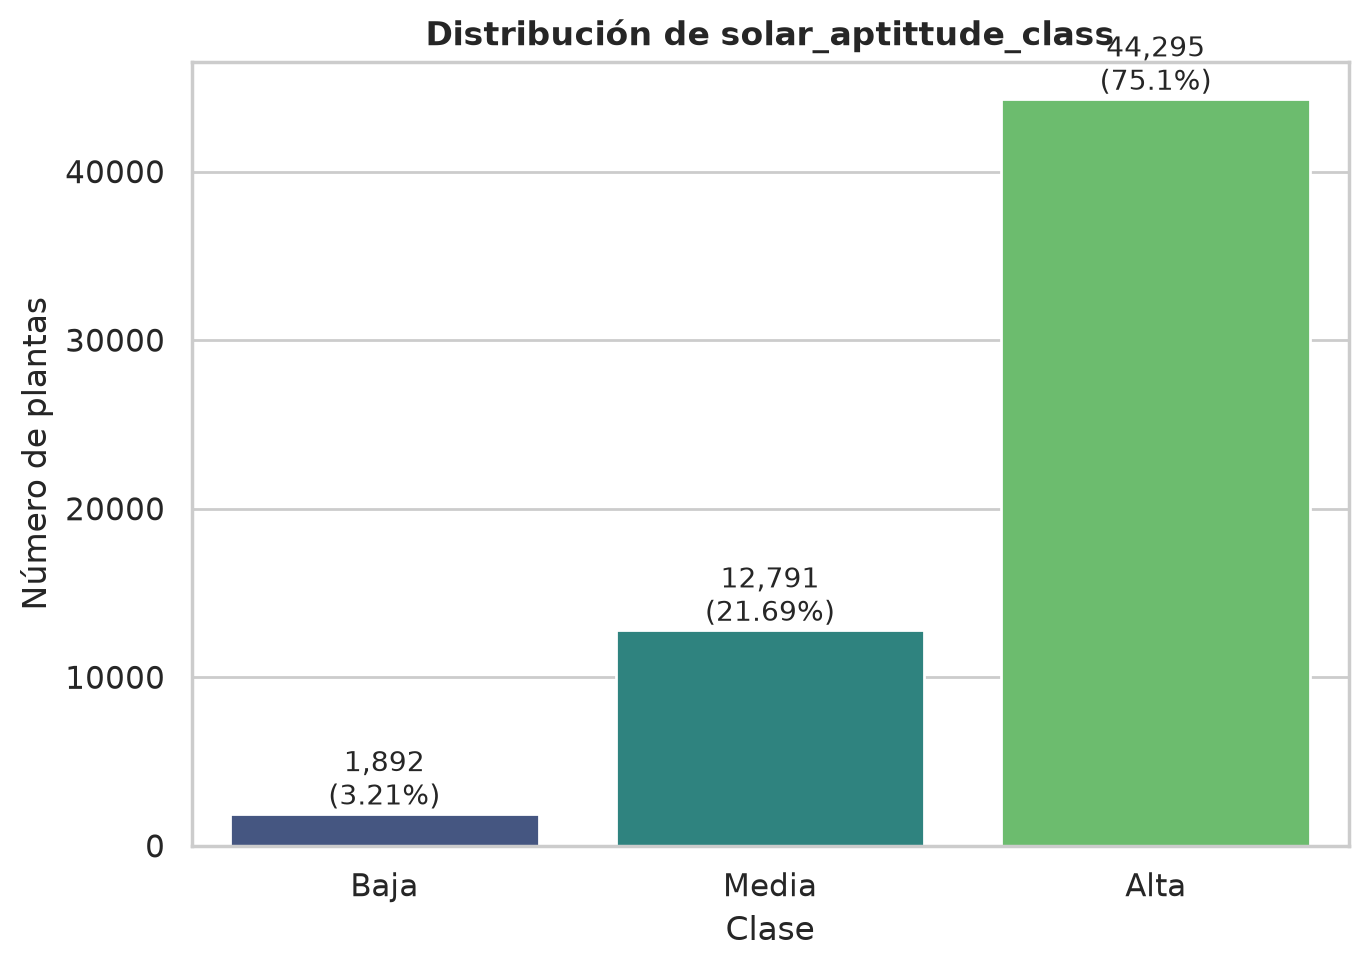
\includegraphics[width=0.6\textwidth]{fig_distribucion_clases.png}
\caption{Distribución de \texttt{solar\_aptittude\_class} sobre las 58{,}978 plantas del dataset. La clase Baja representa apenas el 3.21\% del total.}
\label{fig:clases}
\end{figure}

\subsubsection{Análisis univariado: variables predictoras}\label{subsec:univ_features}

La Tabla~\ref{tab:descriptivas} resume la estadística descriptiva de las 13 variables predictoras numéricas. \texttt{area} (asimetría 72.62) y \texttt{dist\_to\_road} (48.74) presentan las colas más largas: la mediana de \texttt{area} es 8{,}067 pero su máximo supera los 234 millones, evidencia de que unas pocas plantas de escala muy grande dominan la parte superior de la distribución. \texttt{slope} (3.98), \texttt{wind\_speed} (3.56) y \texttt{elevation} (3.18) también están sesgadas a la derecha, mientras que \texttt{latitude} ($-1.96$) y \texttt{humidity} ($-1.49$) lo están a la izquierda.

\begin{table}[h]
\caption{Estadística descriptiva de las 13 variables predictoras numéricas ($n=58{,}978$, salvo \texttt{area} con $n=42{,}649$; 0\% de valores faltantes en el resto).}\label{tab:descriptivas}
\begin{tabular}{@{}lcccccc@{}}
\toprule
Variable & Media & Desv. est. & Mín. & Mediana & Máx. & Asimetría \\
\midrule
longitud (°)          & 43.676   & 77.315   & $-124.104$ & 26.764  & 177.982       & $-0.393$ \\
latitud (°)           & 34.862   & 16.007   & $-41.609$  & 37.012  & 59.939        & $-1.957$ \\
elevación (msnm)      & 353.619  & 526.640  & $-378.000$ & 156.000 & 5656.000      & 3.181 \\
área                  & 180723.2 & 1{,}999{,}936 & 0.013 & 8067.380 & 234{,}700{,}000 & 72.622 \\
pendiente (°)         & 1.454    & 2.258    & 0.000      & 0.674   & 34.682        & 3.983 \\
curvatura             & $-0.0006$& 0.014    & $-0.173$   & 0.000   & 0.270         & 0.547 \\
aspecto (°)           & 171.590  & 98.542   & $-1.000$   & 170.671 & 359.610       & 0.035 \\
distancia a vía (m)   & 3821.722 & 34190.878& 0.000      & 724.383 & 2{,}295{,}655.255 & 48.744 \\
temperatura (°C)      & 14.593   & 5.770    & $-17.064$  & 13.744  & 30.341        & 0.648 \\
irradiancia (kWh/m\textsuperscript{2}) & 4.549 & 0.859 & 0.000 & 4.469 & 8.048 & 0.462 \\
humedad (\%)          & 66.898   & 11.645   & 0.000      & 70.247  & 95.000        & $-1.488$ \\
v. viento (m/s)       & 0.992    & 0.935    & 0.000      & 0.777   & 12.755        & 3.564 \\
d. viento (°)         & 192.966  & 59.192   & 0.000      & 218.604 & 352.500       & $-0.509$ \\
\botrule
\end{tabular}
\end{table}

Las variables categóricas de terreno están dominadas por una sola categoría: \texttt{slope\_type} tiene 79.3\% de plantas en terreno plano o casi plano y \texttt{curvature\_type} tiene 81.1\% en superficies planas o intermedias. \texttt{aspect\_type} está más repartida entre sus ocho orientaciones cardinales (entre 4{,}906 y 8{,}335 plantas cada una), más 1{,}105 plantas (1.9\%) marcadas como \texttt{Flat}. \texttt{dt\_wind}, en cambio, concentra el 73.2\% de los registros en solo tres de sus ocho categorías (\texttt{Southwest}, \texttt{West}, \texttt{Southeast}).

\subsubsection{Análisis geográfico y sesgo de cobertura}\label{subsec:geografico}

Los diez países con más registros concentran el 79.8\% de las 58{,}978 plantas, pese a que el dataset cubre 183 países en total (Tabla~\ref{tab:paises}). La composición de clases varía de forma marcada entre ellos: China, Japón, India, Corea del Sur y Brasil no registran ninguna planta Baja, y Estados Unidos tiene solo una entre sus 7{,}224 plantas, mientras que Alemania, España, Reino Unido y Francia concentran casi toda la representación de esa clase entre los países dominantes. La clase minoritaria del problema es, en la práctica, casi exclusivamente europea dentro de este subconjunto.

\begin{table}[h]
\caption{Los 10 países con más registros, porcentaje del dataset, y composición de clases (\%) de \texttt{solar\_aptittude\_class} dentro de cada país.}\label{tab:paises}
\begin{tabular}{@{}lcccc@{}}
\toprule
País & \% del dataset & Baja & Media & Alta \\
\midrule
China          & 19.53 & 0.0  & 2.4  & 97.6 \\
Japón          & 14.58 & 0.0  & 0.6  & 99.4 \\
Estados Unidos & 12.25 & 0.0  & 56.9 & 43.0 \\
Alemania       & 12.05 & 4.6  & 34.0 & 61.4 \\
India          & 4.93  & 0.0  & 0.2  & 99.8 \\
España         & 4.28  & 8.2  & 32.4 & 59.4 \\
Reino Unido    & 3.87  & 3.2  & 28.7 & 68.1 \\
Corea del Sur  & 3.43  & 0.0  & 0.4  & 99.6 \\
Francia        & 2.46  & 10.4 & 31.0 & 58.6 \\
Brasil         & 2.44  & 0.0  & 37.8 & 62.2 \\
\botrule
\end{tabular}
\end{table}

Esta asociación entre país y clase, junto con el hecho de que \texttt{longitude} obtuvo el estadístico de Kruskal-Wallis más alto de todo el análisis bivariado (Sección~\ref{subsec:bivariado}), sugiere que un modelo entrenado sin cuidado podría aprender a asociar región geográfica con clase de aptitud en lugar de una relación física entre terreno, clima y aptitud. Se recomienda, por tanto, una \textbf{validación cruzada espacial} agrupando por país o continente en las siguientes entregas, en lugar de una partición aleatoria de instancias, para obtener una estimación realista de la capacidad de generalización a ubicaciones no representadas en el dataset \cite{bib2}. La alta cardinalidad de \texttt{country} (183 categorías) hace además poco práctico incorporarlo directamente como predictora categórica sin alguna forma de agregación por región.

\subsubsection{Chequeo de fuga de datos}\label{subsec:leakage}

\texttt{solar\_aptitude} y \texttt{solar\_aptitude\_rounded} separan las tres clases sin superposición (Baja hasta 0.400, Media entre 0.4 y 0.6, Alta desde 0.6), consistente con que son la misma variable de la que se deriva el target por binning. \texttt{capacity}, en cambio, no muestra una diferencia real entre clases (medias de 44.4, 37.8 y 39.4 MW para Baja, Media y Alta, con desviaciones estándar superiores a 300 en los tres casos), y \texttt{pv\_potential} tampoco distingue claramente las clases (3.88, 3.92 y 3.76 kWh/kWp). \texttt{optimal\_tilt} presenta una diferencia más consistente aunque modesta ($33.7^\circ$, $33.1^\circ$ y $30.6^\circ$). La exclusión de estas tres últimas variables se sostiene, entonces, por ser información posterior a la decisión de inversión, y no porque los datos muestren que filtran directamente el target.

\subsubsection{Análisis bivariado y multicolinealidad}\label{subsec:bivariado}

Dado que el target es categórico, la relación de cada feature numérica con \texttt{solar\_aptittude\_class} se evaluó con el test de Kruskal-Wallis \cite{bib4}, y la redundancia entre predictoras con el Factor de Inflación de Varianza (VIF),

\begin{equation}
\mathrm{VIF}_j = \frac{1}{1 - R_j^2},
\label{eq:vif}
\end{equation}

\noindent donde $R_j^2$ es el coeficiente de determinación de la regresión de la variable $j$ sobre el resto de las predictoras \cite{bib5}. La Tabla~\ref{tab:kruskal_vif} muestra que las 13 variables son estadísticamente significativas ($p<0.001$ en todos los casos), aunque con casi 59{,}000 observaciones incluso diferencias pequeñas alcanzan significancia, por lo que la magnitud de $H$ importa más que el umbral de $p$. \texttt{longitude} domina por un margen amplio ($H=12{,}890.78$), lo que es consistente con el sesgo geográfico descrito en la Sección~\ref{subsec:geografico}. En cuanto a multicolinealidad, la Figura~\ref{fig:corr} y la Tabla~\ref{tab:kruskal_vif} muestran que ninguna variable supera un VIF de 4.29 (\texttt{ghi}), muy por debajo del umbral habitual de 10, por lo que no hay evidencia de redundancia severa entre predictoras.

\begin{table}[h]
\caption{Estadístico de Kruskal-Wallis ($H$) frente al target y Factor de Inflación de Varianza (VIF) de las 13 variables predictoras numéricas, ordenadas por $H$ descendente. Todas resultaron significativas ($p<0.001$).}\label{tab:kruskal_vif}
\begin{tabular}{@{}lcc@{}}
\toprule
Variable & $H$ (Kruskal-Wallis) & VIF \\
\midrule
longitud         & 12890.78 & 1.276 \\
pendiente        & 3712.68  & 1.176 \\
distancia a vía  & 2605.13  & 1.011 \\
latitud          & 2175.86  & 3.402 \\
elevación        & 1395.65  & 1.960 \\
v. viento        & 1332.86  & 1.817 \\
temperatura      & 785.22   & 3.070 \\
d. viento        & 445.48   & 1.234 \\
área             & 341.06   & 1.015 \\
irradiancia      & 166.88   & 4.292 \\
humedad          & 112.35   & 2.360 \\
aspecto          & 22.41    & 1.004 \\
curvatura        & 19.54    & 1.014 \\
\botrule
\end{tabular}
\end{table}

\begin{figure}[h]
\centering
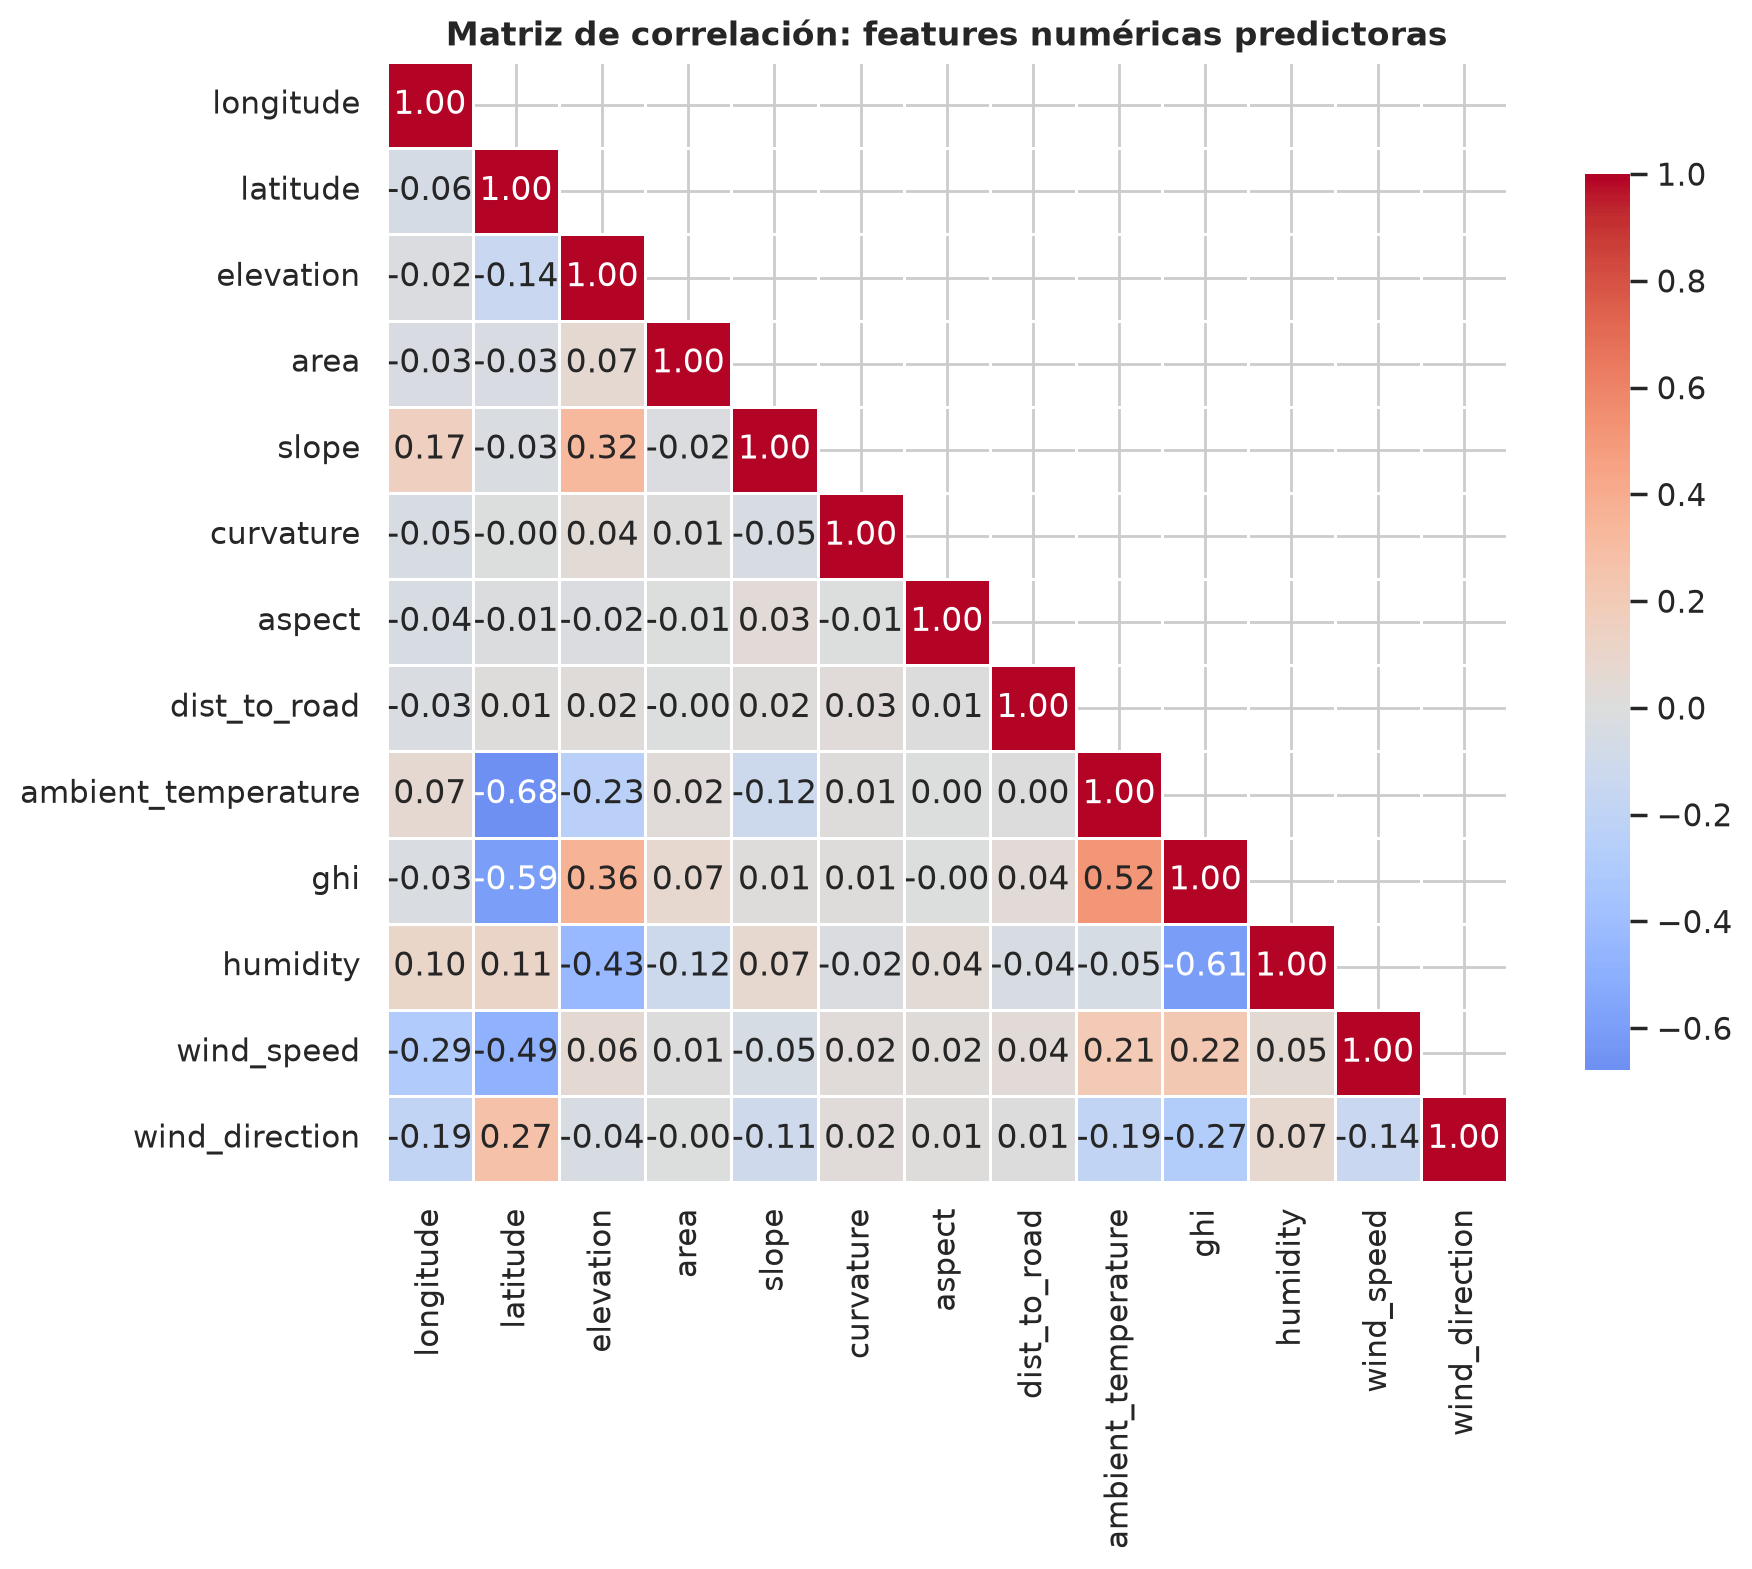
\includegraphics[width=0.85\textwidth]{fig_correlacion.png}
\caption{Matriz de correlación de Pearson entre las 13 variables predictoras numéricas.}
\label{fig:corr}
\end{figure}

\subsubsection{Detección de outliers}\label{subsec:outliers}

Se aplicó el método de rango intercuartílico (IQR, factor 1.5) a las 13 variables numéricas (Tabla~\ref{tab:outliers}, Figura~\ref{fig:outliers}). \texttt{curvature} presenta la mayor proporción de valores atípicos (18.95\%), aunque en gran parte por un artefacto del método: la variable está tan concentrada cerca de cero que su rango intercuartílico es minúsculo y cualquier desviación moderada queda marcada como atípica. \texttt{area} (13.53\%) y \texttt{dist\_to\_road} (12.78\%), en cambio, sí reflejan una cola larga genuina: 1{,}261 plantas superan por sí solas el millón de unidades de área. \texttt{longitude}, \texttt{aspect} y \texttt{wind\_direction} no presentan ningún outlier bajo este criterio.

\begin{table}[h]
\caption{Resumen de detección de outliers (método IQR, factor 1.5), ordenado por porcentaje de outliers.}\label{tab:outliers}
\begin{tabular}{@{}lccc@{}}
\toprule
Variable & N.\textsuperscript{o} outliers & \% outliers & Límites [inf., sup.] \\
\midrule
curvatura        & 11{,}174 & 18.95 & $[-0.010,\ 0.009]$ \\
área             & 5{,}770  & 13.53 & $[-90224.620,\ 153468.964]$ \\
distancia a vía  & 7{,}539  & 12.78 & $[-3442.272,\ 6308.168]$ \\
pendiente        & 5{,}633  & 9.55  & $[-1.884,\ 3.785]$ \\
elevación        & 5{,}459  & 9.26  & $[-536.000,\ 1016.000]$ \\
latitud          & 4{,}632  & 7.85  & $[12.712,\ 63.231]$ \\
humedad          & 3{,}362  & 5.70  & $[44.166,\ 92.899]$ \\
v. viento        & 3{,}099  & 5.25  & $[-0.554,\ 2.258]$ \\
temperatura      & 644    & 1.09  & $[-0.478,\ 27.941]$ \\
irradiancia      & 112    & 0.19  & $[1.749,\ 7.330]$ \\
longitud         & 0      & 0.00  & $[-178.621,\ 295.038]$ \\
aspecto          & 0      & 0.00  & $[-155.108,\ 498.513]$ \\
d. viento        & 0      & 0.00  & $[-26.942,\ 403.082]$ \\
\botrule
\end{tabular}
\end{table}

\begin{figure}[h]
\centering
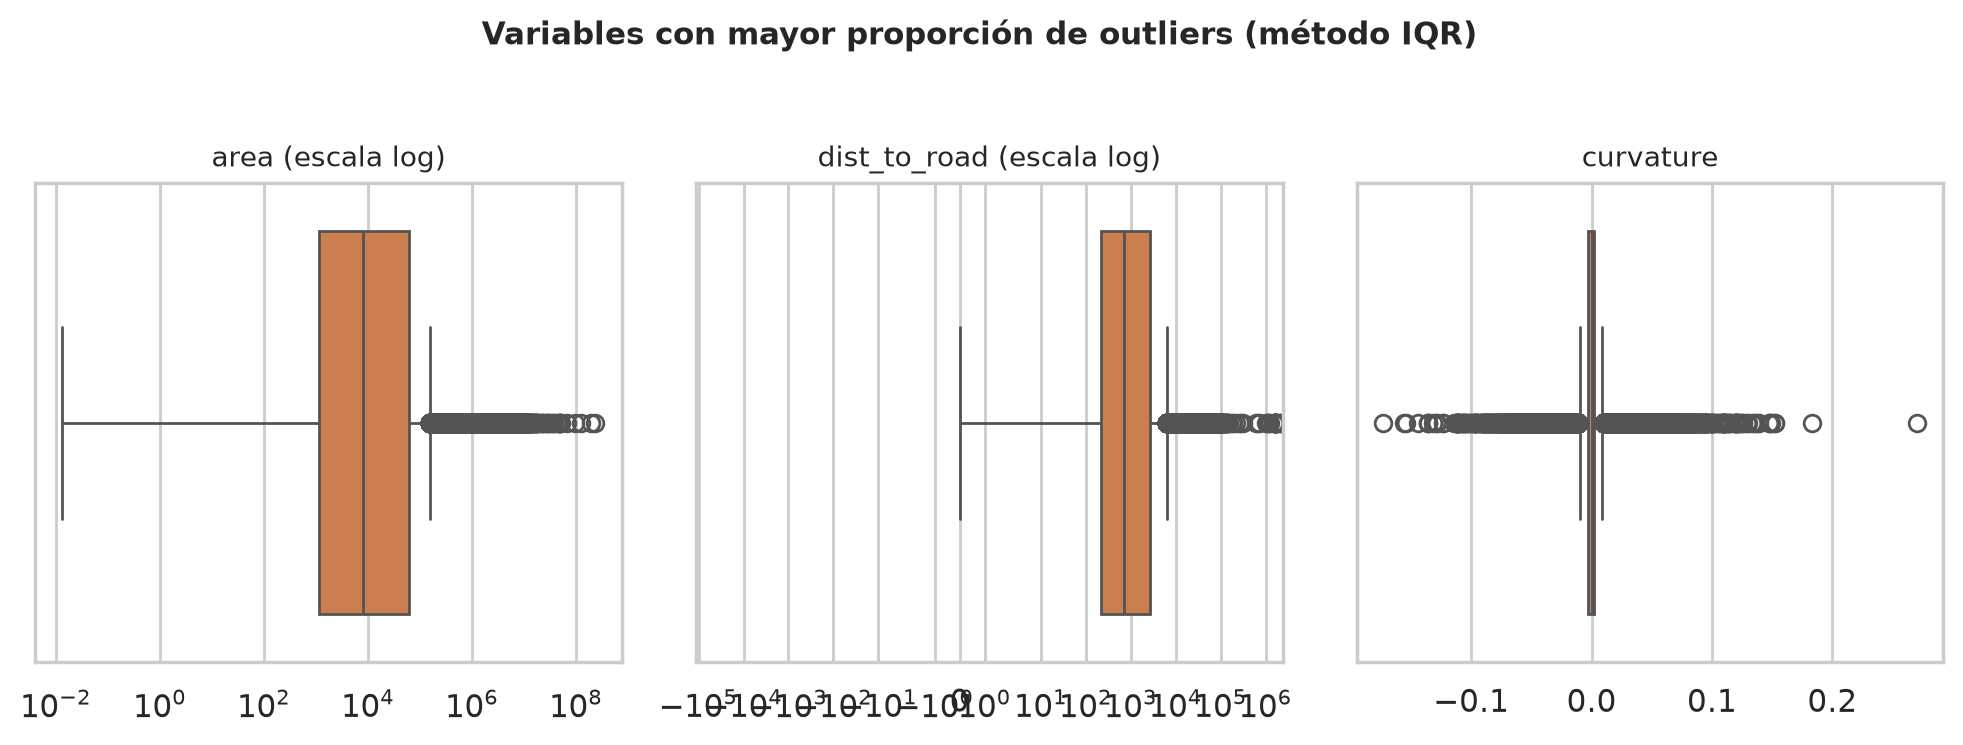
\includegraphics[width=0.95\textwidth]{fig_outliers.png}
\caption{Boxplots de las tres variables con mayor proporción de outliers según el método IQR.}
\label{fig:outliers}
\end{figure}

\subsubsection{Segmentación adicional}\label{subsec:segmentacion}

\texttt{size} (\texttt{Small} 69.6\%, \texttt{Medium} 22.4\%, \texttt{Big} 8.0\%) varía con el estado operacional de la planta: \texttt{operating} tiene 7.9\% de plantas \texttt{Big} y 24.5\% \texttt{Medium}, mientras que \texttt{pre-construction} tiene una proporción similar de \texttt{Big} (8.2\%) pero muchas menos \texttt{Medium} (9.7\%). Esto sugiere que \texttt{size} codifica al menos parcialmente el tamaño del proyecto ya construido, y no únicamente el terreno disponible antes de invertir. La segmentación por banda climática confirma el patrón esperado: la banda tropical norte concentra 87.2\% de aptitud Alta, frente a 55--58\% en las bandas templadas y tropical sur.

\subsubsection{Conclusiones del EDA y decisiones de preprocesamiento}\label{subsec:conclusiones_eda}

El EDA exhaustivo permite consolidar las siguientes decisiones de preprocesamiento, cada una derivada directamente de un hallazgo cuantitativo de esta sección:

\begin{itemize}
\item \textbf{Desbalance de clases:} con Baja representando el 3.21\% del dataset, el modelado usará métricas sensibles al desbalance (F1 macro, recall por clase), partición estratificada, y ponderación de clases o remuestreo durante el entrenamiento (Sección~\ref{subsec:univ_target}).
\item \textbf{Validación cruzada espacial:} dado que 10 países concentran el 79.8\% de los registros y la clase Baja está casi enteramente concentrada en Europa, la evaluación de modelos usará bloques geográficos en lugar de una partición aleatoria (Sección~\ref{subsec:geografico}).
\item \textbf{Codificación cíclica de variables angulares:} \texttt{aspect} y \texttt{wind\_direction} se transforman a pares seno/coseno en lugar de usarse como grados crudos (Sección~\ref{subsec:etl}).
\item \textbf{Exclusión de variables de fuga y posteriores a la inversión:} \texttt{solar\_aptitude}, \texttt{solar\_aptitude\_rounded}, \texttt{capacity}, \texttt{optimal\_tilt}, \texttt{pv\_potential} y \texttt{operational\_status} se excluyen del conjunto de \emph{features} (Sección~\ref{subsec:leakage}).
\item \textbf{Sin corrección adicional de multicolinealidad:} con un VIF máximo de 4.29, no se requiere excluir ni combinar variables numéricas antes de un modelo lineal (Sección~\ref{subsec:bivariado}).
\item \textbf{Tratamiento de outliers según variable:} \texttt{area} y \texttt{dist\_to\_road}, con colas genuinamente largas, favorecen modelos robustos a outliers (árboles, ensambles) sobre una regresión lineal sin tratamiento previo; el alto porcentaje de \texttt{curvature} se atribuye al método y no requiere recorte (Sección~\ref{subsec:outliers}).
\item \textbf{Decisiones pendientes para la siguiente entrega:} imputación de \texttt{area} (27.69\% de nulos), codificación de \texttt{country} y \texttt{size}, y codificación categórica (one-hot u ordinal) de \texttt{slope\_type}, \texttt{curvature\_type}, \texttt{aspect\_type} y \texttt{dt\_wind}.
\end{itemize}

\section*{Referencias bibliográficas}

\begin{thebibliography}{99}

\bibitem{bib1} Mantilla-Guerra, A., Mejia-Escobar, C., Azorin-Lopez, J., Garcia-Rodriguez, J., Tarco, B.F., Santamaria, K.: Global Dataset of Solar Power Plants: Multidimensional Integration and Analysis. arXiv:2603.20601 (2026)

\bibitem{bib2} Roberts, D.R., Bahn, V., Ciuti, S., Boyce, M.S., Elith, J., Guillera-Arroita, G., Hauenstein, S., Lahoz-Monfort, J.J., Schröder, B., Thuiller, W., Warton, D.I., Wintle, B.A., Hartig, F., Dormann, C.F.: Cross-validation strategies for data with temporal, spatial, hierarchical, or phylogenetic structure. Ecography \textbf{40}(8), 913--929 (2017)

\bibitem{bib3} James, G., Witten, D., Hastie, T., Tibshirani, R.: An Introduction to Statistical Learning, 2nd edn. Springer, New York (2021)

\bibitem{bib4} Kruskal, W.H., Wallis, W.A.: Use of Ranks in One-Criterion Variance Analysis. Journal of the American Statistical Association \textbf{47}(260), 583--621 (1952)

\bibitem{bib5} Kutner, M.H., Nachtsheim, C.J., Neter, J., Li, W.: Applied Linear Statistical Models, 5th edn. McGraw-Hill/Irwin, New York (2005)

\end{thebibliography}

\end{document}
